\chapter{Cross Travel Manual Screen}
\begin{figure}
	\centering
	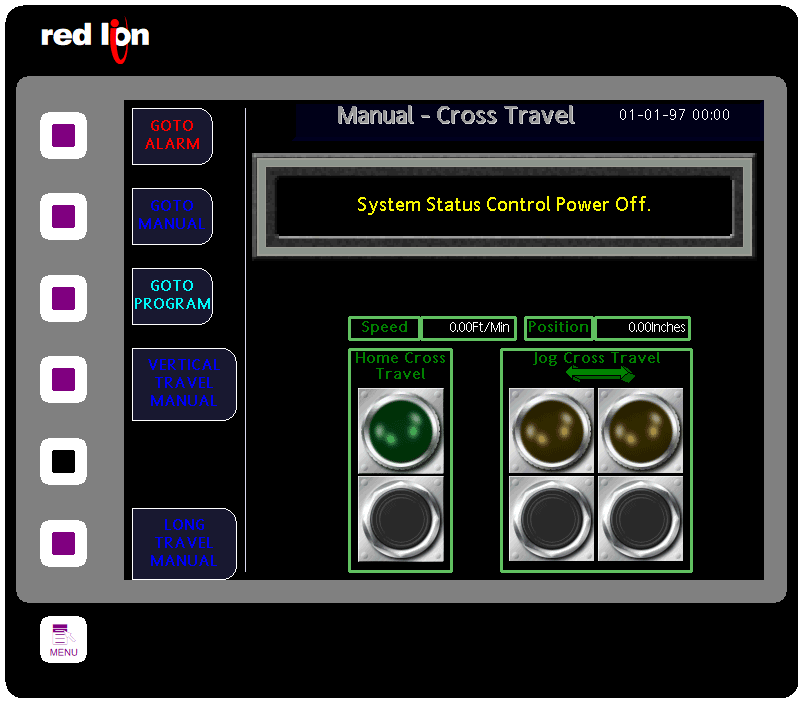
\includegraphics[width=0.5\linewidth]{screen-captures/manual/trans-manual}
	\caption{Cross Travel Manual Screen}
	\label{fig:manual-cross-screen}
\end{figure}
\section{Overview}\paragraph*{The}\textbf{Cross Travel} manual screen (Figure 5.1) provides the Operator access to control the \textbf{Cross Travel} axis while in \textit{Hand} mode. The Operator is able to initiate a homing function, and there are indicators for \textbf{At Home}, plus while in motion. Navigation is possible to the main \textbf{Manual} screen, the \textbf{Cut Program} screen, both the \textbf{Vertical} and \textbf{Long Axis} manual screens, and of course the \textbf{Main} operation screen.
\section{Details}\paragraph*{The}\textbf{Cross Travel Manual} screen details are divided into the following categories ...
\begin{list}{$\diamond$}{}
	\item \textbf{Screen Navigation}
	\item \textbf{Cross Travel Home}
	\item \textbf{Cross Travel Control}
\end{list}
\begin{figure}
	\centering
	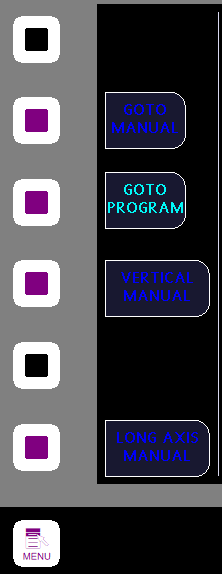
\includegraphics[width=0.2\linewidth]{screen-captures/manual/trans-manual-nav}
	\caption{Cross Travel Manual Screen Navigation}
	\label{fig:manual-cross-screen-nav}
\end{figure}
\subsection{Screen Navigation}\paragraph*{Is}performed by using the programmable Function Keys (FKeys) located down the left hand side of the OI Terminal (refer to Figure 5.2). The Operator may navigate to the following screens ...
\begin{list}{$\diamond$}{}
	\item \textbf{GOTO Alarm} Navigate to Alarm Screen.
	\item \textbf{GOTO MANUAL} Navigate to Manual Screen.
	\item \textbf{GOTO PROGRAM} Navigate to Cut Program Screen.
	\item \textbf{VERTICAL MANUAL} Navigate to Vertical Manual Control Screen.
	\item \textbf{LONG AXIS MANUAL} Navigate to the Long Axis Manual Control Screen.
\end{list}
\paragraph{\textbf{\LARGE \textcolor{blue}{i}}}
The Menu Key located on the terminal at the lower left below the FKey's, will return the Operator to the Main Screen, from all other screens.\\
\begin{minipage}{4cm}
	\begin{picture}(20,70)
	
\includegraphics[width=.5\linewidth]{screen-captures/menu}
	\end{picture}
\end{minipage}\begin{minipage}[]{11cm}
	\paragraph{\textbf{\LARGE \textcolor{blue}{i}}} The Menu Key is pictured as it looks on the Terminal.
\end{minipage}
\subsection{Cross Travel Home}\paragraph*{Home}Function is the stand alone homing routine for the \textbf{Cross Travel} axis. There is a \textbf{Control} pushbutton to initiate the homing function and an \textbf{Indicator} pilot light to indicate when the \textbf{Cross Travel} axis is in the \textbf{Home} position and has completed a homing function. On the saw the \textbf{Cross Travel} axis has it's \textbf{Home} position at the travel limit sensor closest to the Control Panel. A homing function will cause the axis to move in either direction depending upon the state of the \textbf{Home} sensor. If the \textbf{Home} sensor is off, the \textbf{Home} function will command the \textbf{Cross Travel} axis to move towards the operator up to the point the (home) sensor comes on.
\begin{figure}
	\centering
	
\includegraphics[width=.2\linewidth]{screen-captures/manual/trans-manual-home}
	\caption{Cross Travel Manual Home Function}
	\label{fig:cross-manual-home}
\end{figure}
\pagebreak
\subsection{Cross Travel Positioning}
\paragraph*{}Figure 5.4 shows the \textbf{Cross Travel Command} function. The function is made up of a pushbutton to command \textbf{Cross Travel Forward} with a corresponding \textbf{Indicator} pilot light that indicates motion commanded but not complete. There is also a related \textbf{Cross Travel Reverse} pushbutton and \textbf{Indicator}. Finally, there is a position feedback display area which shows the current axis position in inches and it's velocity in feet per minute. This function is available in \textit{Hand} mode and is intended for use by the Operator during Machine Setup and Maintenance activities.
\begin{figure}
	\centering
	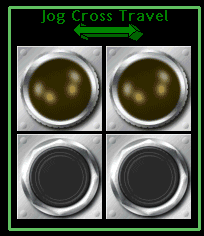
\includegraphics[width=.2\linewidth]{screen-captures/manual/trans-manual-command}
	\caption{Cross Travel Manual Command}
	\label{fig:cross-manual-command}
\end{figure}
\begin{figure}
	\centering
	
\includegraphics[width=.2\linewidth]{screen-captures/manual/trans-manual-fdbk}
	\caption{Cross Travel Manual Feedback}
	\label{fig:cross-manual-fdbk}
\end{figure} 
\paragraph{\textbf{\LARGE \textcolor{blue}{i}}}The position feedback should be considered invalid if the axis has not been homed yet, since the position encoder is an incremental encoder and does not retain position information on a power cycle. Therefore it is required to reference the axis feedback to zero on successful homing completion, in order to ensure positional accuracy and repeatability.
